\documentclass[12pt]{article}
\usepackage[margin=0.75in]{geometry}
\usepackage{graphicx}
\usepackage{tabularx}
\usepackage{times}
\usepackage[T1]{fontenc}
\usepackage{textcomp}
\usepackage{titlesec}
\usepackage{fancyvrb}
\usepackage{parskip}
\usepackage{array, booktabs}
\usepackage{caption}
\usepackage{subcaption}

\titleformat{\section}{\large\bfseries}{\thesection.}{0.5em}{}
\titleformat{\subsection}{\normalsize\bfseries}{\thesection.}{0.5em}{}
\titlespacing{\section}{0em}{1em}{0em}
\titlespacing{\subsection}{0em}{0.25em}{0em}
\newcolumntype{C}{>{\centering\arraybackslash}X}


\graphicspath{ {img/} }

\begin{document}

{\centering\Large
  \textbf{\texttt{mc}: A Compiler for the ``Mini'' Language}\\
         {\normalsize{\em CPE431 Final Report} / Jacob Hladky / \today}
         \par
}

\vspace{0.5cm}

Mc is a compiler for the ``mini'' toy language, targeting the amd64 architecture on OS X and GNU/Linux. Mc is written entirely in SML, and depends on one external SML module: ``SML-JSON'', which provides callbacks that assist in parsing. Mc produces either an ELF or a MachO object file that is assembled and linked by the GNU assembler and linker.

The program ``mc'' is in fact a bash script which handles command-line argument parsing and which calls the SML ``compiler'' binary along with any other required programs. The ``compiler'' binary is itself compiled with mlton.

\section*{Architecture}
Mc is input with a source file containing a JSON-representaion of the AST for a mini program, and parses this JSON into an internal AST with the \texttt{json2Ast} function. Then it scans through the AST to collect various information about the program. This information is collected into the symbol table using the \texttt{mkSymbolTable} function.

The AST and symbol table are then passed into the static checker. The \texttt{staticCheck} function runs a series of tests on the program to make sure that it does not violate the semantics of the source language. All type checking is done in this step. The static checker can fail; upon failure the checker prints an error message and compilation stops. After the static checker finishes compilation is guaranteed.

The AST and symbol table are then converted to the ILOC intermediary assembly using the \texttt{ast2Iloc} function. The ILOC is then run through several optimizing steps, detailed below. After being optimized the ILOC is converted to amd64 assembly using virtual registers with the \texttt{iloc2Amd64} function. Register allocation is then performed by the \texttt{regAlloc} function.

This completes the compilation process. The resulting amd64 assembly is outputted using the \texttt{programToStr} function. The resulting object file is then assembled and linked.

\section*{Internal Structures}
\subsection*{AST}
The structure of the AST is defined by the JSON input file. The only notable feature of mc's AST is that all nodes preserve line numbers so that they can be presented to the user if there is an error from static analysis.

\subsection*{Symbol Table}
The symbol table is one of the most important data structures in mc. It consists of two custom data-types with the following definitions:

\begin{figure}
\centering
\begin{BVerbatim}[fontsize=\scriptsize]
datatype func_info =
    FUNC_INFO of {
        params: Ast.typ list,
        returnType: Ast.typ,
        calls: string list
    }

datatype symbol_table =
    ST of {
        types: (string, (string, Ast.typ) HashTable.hash_table)
            HashTable.hash_table,
        globals: (string, Ast.typ) HashTable.hash_table,
        funcs: (string, func_info) HashTable.hash_table,
        locals: (string, (string, Ast.typ) HashTable.hash_table)
            HashTable.hash_table
    }
\end{BVerbatim}
\caption{Datatypes used in the symbol table.}
\end{figure}

The \texttt{types} field is used by the static checker to verify type correctness. It is also used when converting the AST to the ILOC to calculate structure access offsets. The \texttt{funcs} field is used determine whether it is necessary to add spill space to functions when converting the ILOC to amd64. The remaining fields are only used by the static checker.

\subsection*{Control Flow Graph}
The control flow graph is implemented generically, and is used to represent the ILOC and the amd64 assembly. It implements several of the higher-order functions, including map, fold, and apply. The CFG significant use of references and thus mutation, and although it purports a functional interface, it is not implemented functionally. This implementation, although ugly, is simpler and solves several issues when optimizing the ILOC.

\subsection*{Interference Graph and Virtual-To-Real map}
The interference graph is undirected and was significantly easier to implement. Like the CFG, it supports the higher-order functions, but it is not implemented generically, because it is only used for register allocation. The Virtual-To-Real map is a hash table that is used to keep track of how virtual registers map to real registers. It is used in conjunction with the interference graph during register allocation: the interference graph is ``deconstructed'' into a stack and ``reconstructed'' into the virtual-to-real map.

\subsection*{ILOC and Amd64}
The ILOC and Amd64 are each written similarly. Each contains an ``instruction'' datatype and an ``opcode'' datatype. However the ILOC represents registers as integers, while the amd64 represents them as a separate datatype. This is necessary in order to maintain the virtual/real register distinction.

\section*{Optimizations}
The following optimizations are implemented by mc:

\begin{itemize}
\item Copy Propagation (\texttt{copyProp.sml})
\item Local Value Numbering (\texttt{lvNumbering.sml})
\item Dead Code Removal (\texttt{stripDeadCode.sml})
\end{itemize}

The copy propagation and dead code removal optimizations (and the register allocation algorithm) share a common datatype, the \texttt{dataflow\_analysis} structure (\texttt{dfa.sml}). This structure standardizes running the dataflow analysis parts of those algorithms. All functions that use the dfa struct follow the exact same sequence:
\begin{enumerate}
\item Take in a CFG representing the function
\item Initialize any global data needed before-hand, e.g. all copies made in the function, or all definitions
\item Map the basic\_block CFG to a dataflow\_analysis CFG, and pass this in to the \texttt{buildDFAs} function, provided by the dfa struct.
\item Map the resulting dataflow\_analysis CFG back into a basic\_block, in the process the replacement step.
\end{enumerate}
The following block of code from the copyProp module demonstrates this procedure:

\begin{figure}[h!]
\centering
\begin{BVerbatim}[fontsize=\scriptsize]
  fun optFunc (id, cfg) =
    let
        val copies = Cfg.fold findCopies (empty ()) cfg
        val dfas = buildDFAs propagate (Cfg.map (bbToDFA copies) cfg)
    in
        (id, Cfg.map replaceCopies dfas)
    end
\end{BVerbatim}
\caption{Top-level function for the copy propagation optimization}
\end{figure}

The local value numbering optimization does not use dataflow analysis. It optimizes each basic block by numbering values and replacing redundant computations with moves. Local value numbering is the first optimization run, as it generates several (possibly redundant) move instructions. Copy propagation is then run to eliminate these moves, and dead code removal is run last to clean up any more unnecessary code.


%% • Provide a section detailing the performance of the code generated for the benchmarks. This section must
%% contain graphs comparing the run-times of the generated code (with and without optimizations) and the
%% C equivalent code compiled using gcc or clang (with and without optimizations).
\section*{Code Performance}
The optimized code generated by mc was compared to unoptimized code also generated by mc, as well as to optimized and unoptimized code generated by clang. Code was compared based on run-time.

\subsection*{Optimization Notes}
\begin{itemize}
\item The following benchmarks were modified to make them run longer:
\begin{itemize}
\item BenchMarkishTopics
\item OptimizationBenchmark
\item hailstone
\item wasteOfCycles
\end{itemize}
The run-times of these benchmarks with the benchmarks was measured to be 0 seconds by \textit{time} for all cases. By making the code run longer the optimized and unoptimized code could be better compared.
\item clang comparisons were performed against version ``Apple LLVM 6.1.0'' using -O3 for optimized code.
\item All run-time results listed are an average of 10 trials and are in seconds. Only user time was measured. Tests were run on an Intel 2.7 GHz Core-i7 CPU.
\end{itemize}

\subsection*{Results}
Table~\ref{table:time_results} summarizes the results.

\begin{table}[h!]
  \centering
  \begin{tabularx}{0.8\textwidth}{l|CCCC}
    \hline
    \textbf{Benchmark} & \textbf{\texttt{mc} unopt} & \textbf{\texttt{mc} opt} & \textbf{\texttt{clang} unopt} & \textbf{\texttt{clang} opt} \\ \hline
    BenchMarkishTopics      & 01.9030 & 01.9350 & 02.4870 & 00.5940 \\
    TicTac                  & 00.0000 & 00.0000 & 00.0000 & 00.0000 \\
    binaryConverter         & 01.4950 & 01.3910 & 02.5910 & 00.0000 \\
    hailstone               & 00.0000 & 00.0000 & 00.0000 & 00.0000 \\
    mile1                   & 00.0100 & 00.0100 & 00.0100 & 00.0000 \\
    programBreaker          & 00.0000 & 00.0000 & 00.0000 & 00.0000 \\
    wasteOfCycles           & 06.2440 & 06.5360 & 06.3320 & 06.3030 \\
    Fibonacci               & 02.2390 & 02.2370 & 01.7580 & 01.0620 \\
    OptimizationBenchmark   & 01.9790 & 01.5100 & 02.0570 & 00.0000 \\
    bert                    & 00.0000 & 00.0000 & 00.0000 & 00.0000 \\
    creativeBenchMarkName   & 08.6800 & 08.0130 & 16.8790 & 00.0000 \\
    hanoi\_benchmark        & 07.0090 & 06.8410 & 04.1040 & 01.9980 \\
    mixed                   & 01.1380 & 00.7170 & 01.2540 & 00.0000 \\
    stats                   & 00.0000 & 00.0000 & 00.0000 & 00.0000 \\
    GeneralFunctAndOptimize & 01.3810 & 01.1260 & 01.2870 & 00.1770 \\
    biggest                 & 00.0000 & 00.0000 & 00.0000 & 00.0000 \\
    fact\_sum               & 00.0000 & 00.0000 & 00.0000 & 00.0000 \\
    killerBubbles           & 02.1250 & 02.2140 & 02.2910 & 00.8940 \\
    primes                  & 00.1500 & 00.1590 & 00.2230 & 00.1000 \\
    uncreativeBenchmark     & 00.0000 & 00.0000 & 00.0000 & 00.0000 \\
  \end{tabularx}
  \caption{Run-time results}
  \label{table:time_results}
\end{table}

%% \begin{table}[h!]
%%   \centering
%%   \begin{tabulary}{0.8\textwidth}{|l|R|R|R|R|}
%%     \hline
%%     \textbf{Benchmark} & \textbf{\texttt{mc} unopt} & \textbf{\texttt{mc} opt} & \textbf{\texttt{clang} unopt} & \textbf{\texttt{clang} opt} \\ \hline\hline
%%     BenchMarkishTopics      & 08.824 & 0.0824 & & \\ \hline
%%     TicTac                  & 12.968 & 12.968 & & \\ \hline
%%     binaryConverter         & 08.760 & & & \\ \hline
%%     hailstone               & 08.648 & & & \\ \hline
%%     mile1                   & 08.656 & & & \\ \hline
%%     programBreaker          & 08.704 & & & \\ \hline
%%     wasteOfCycles           & 08.608 & & & \\ \hline
%%     Fibonacci               & 08.608 & & & \\ \hline
%%     OptimizationBenchmark   & 13.792 & & & \\ \hline
%%     bert                    & 13.664 & & & \\ \hline
%%     creativeBenchMarkName   & 08.792 & & & \\ \hline
%%     hanoi\_benchmark        & 08.912 & & & \\ \hline
%%     mixed                   & 08.396 & & & \\ \hline
%%     stats                   & 08.832 & & & \\ \hline
%%     GeneralFunctAndOptimize & 08.784 & & & \\ \hline
%%     biggest                 & 08.744 & & & \\ \hline
%%     fact\_sum               & 08.632 & & & \\ \hline
%%     killerBubbles           & 08.824 & & & \\ \hline
%%     primes                  & 08.640 & & & \\ \hline
%%     uncreativeBenchmark     & 08.768 & & & \\ \hline
%%   \end{tabulary}
%%   \caption{Output binary size results}
%%   \label{table:size_results}
%% \end{table}

\subsection*{Analysis}
Table~\ref{table:time_results} shows that several benchmarks, despite having their inputs modified, still registered 0 user time. Meaningful comparison for these benchmarks is not possible.

\begin{figure}[ht!]
  \centering
  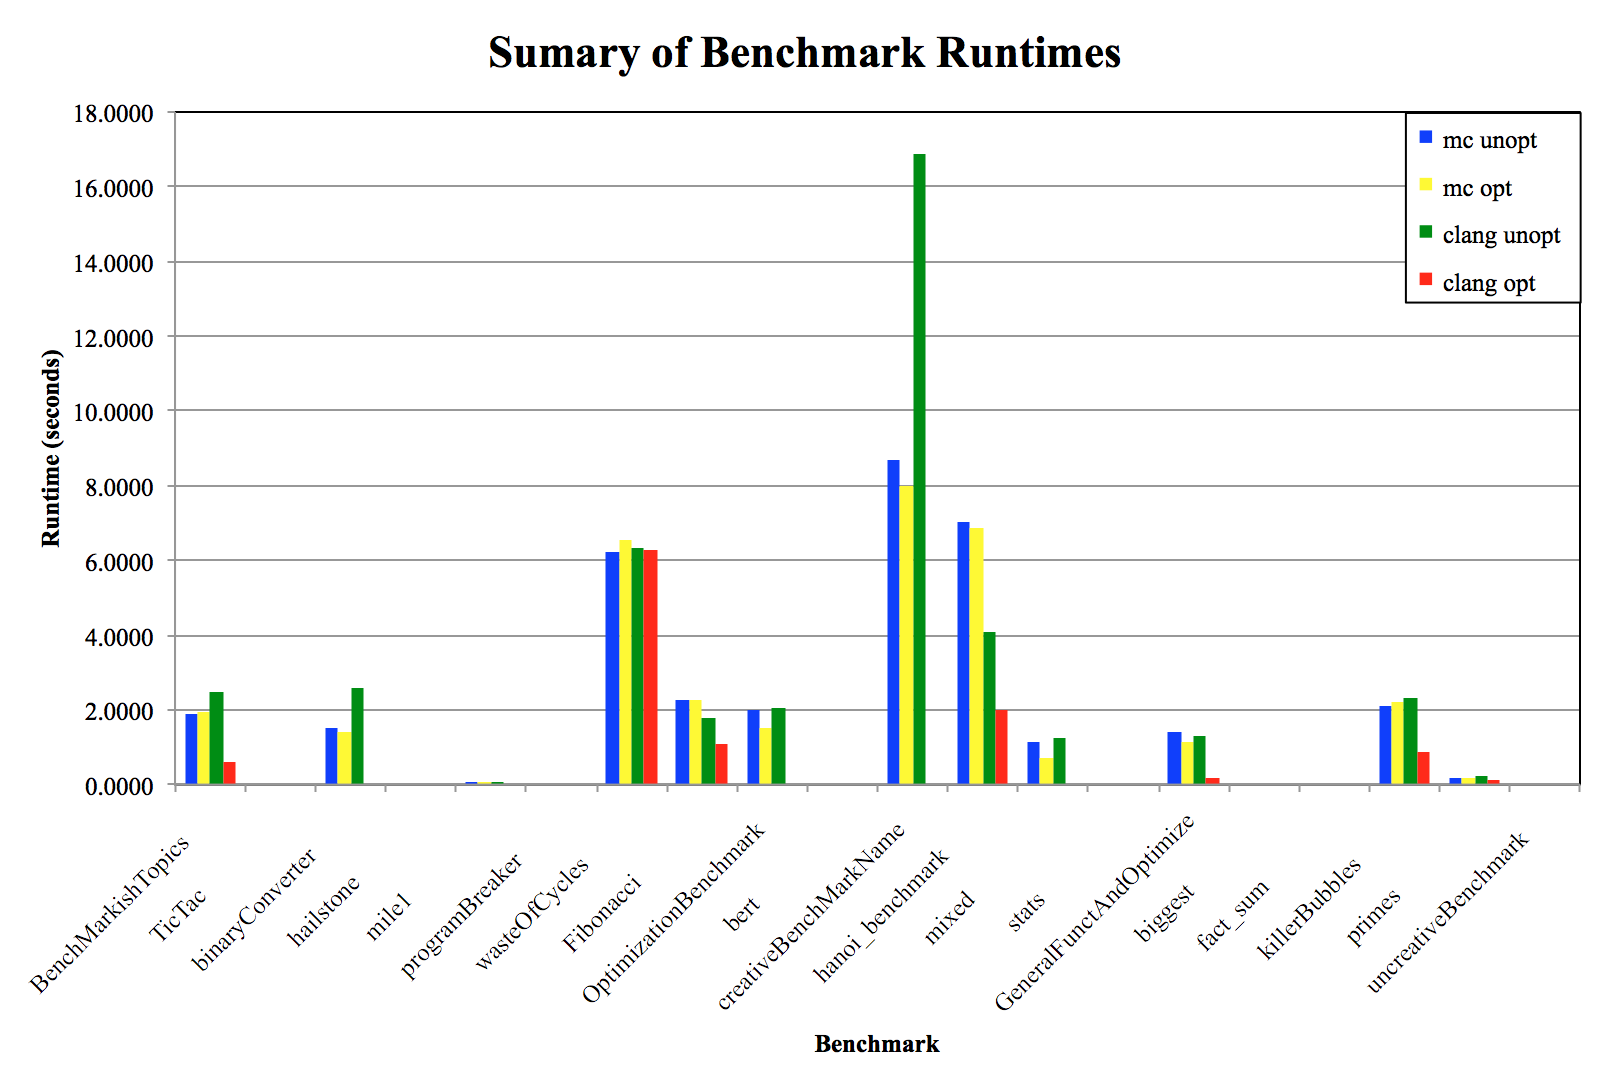
\includegraphics[width=\textwidth]{summary.png}
  \caption{Summary of results}
  \label{fig:summary}
\end{figure}

\begin{figure}
\centering
\begin{subfigure}{.5\textwidth}
  \centering
  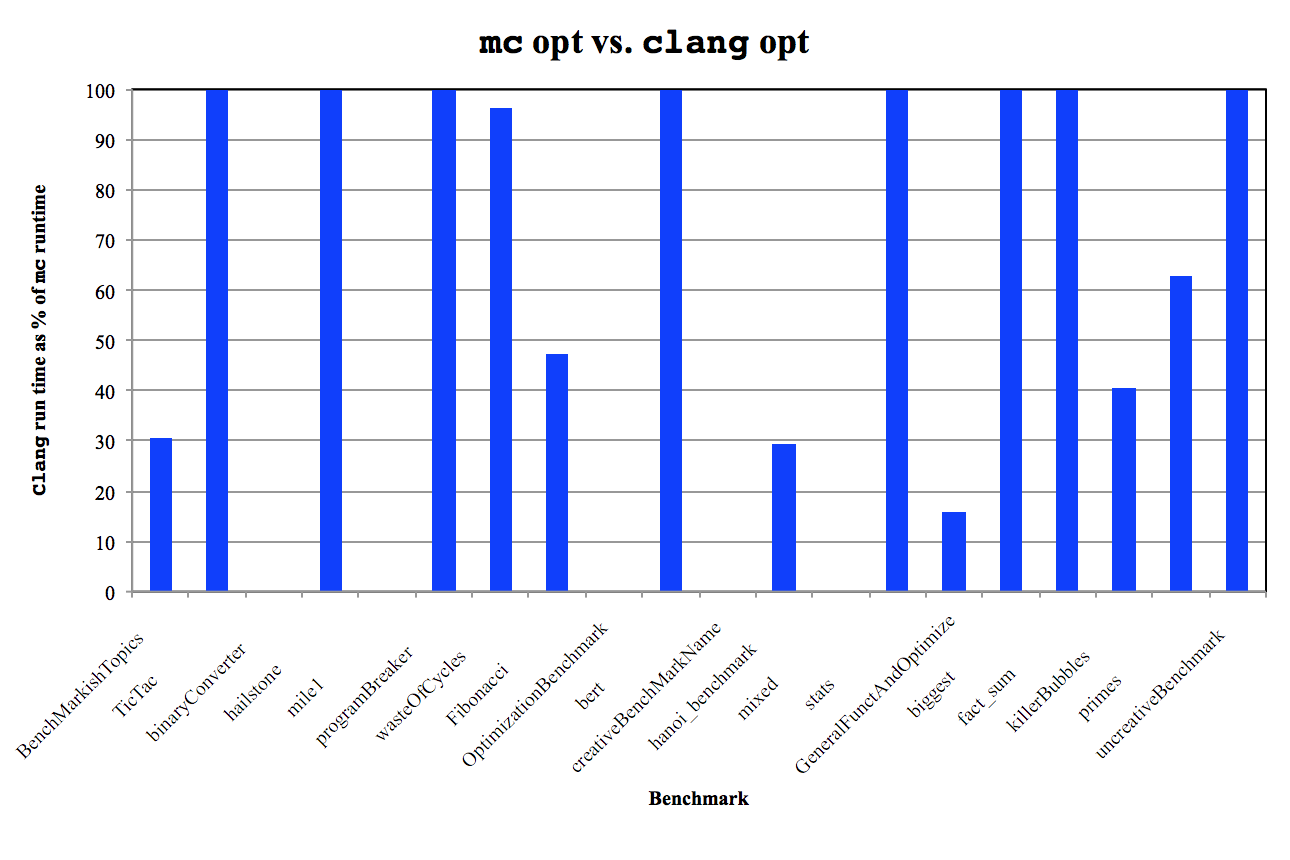
\includegraphics[width=.95\linewidth]{opt.png}
  \caption{With optimizations.}
  \label{fig:opt}
\end{subfigure}%
\begin{subfigure}{.5\textwidth}
  \centering
  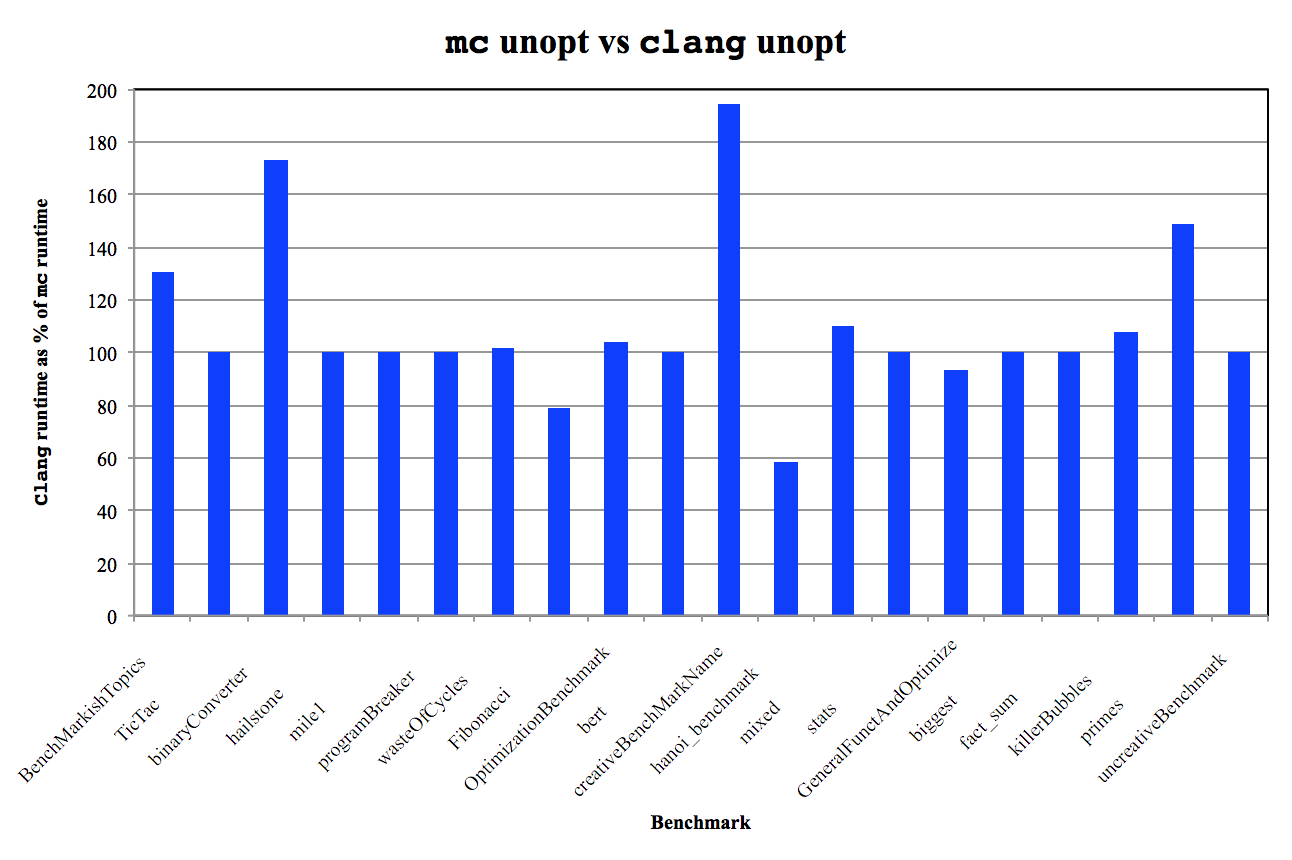
\includegraphics[width=.95\linewidth]{unopt.png}
  \caption{Without optimizations}
  \label{fig:unopt}
\end{subfigure}
\caption{\texttt{Mc} vs \texttt{clang}}
\label{fig:vs}
\end{figure}

\end{document}
